\graphicspath{{Img/slingshot/}}

\chapter{Slingshot}

\section{Assignment}
The work performed in this thesis follows closely the work, which I did in the subject called ``Individual project''~\cite{PreDiplomaLejsekHlavac}, where I focused on exploring the possibilities of a robotic slingshot. Here I continue with developing a fully automated slingshot.
	
The goal is to implement the following shooting procedure. The right arm holds the projectile and the slingshot is attached to the left one.
%
		\begin{enumerate}\itemsep0pt
		    \item Load the projectile. Use force feedback to determine that the elastic string has been touched.
		    \item Stretch the elastic string of the slingshot by moving the attached projectile using the right arm. Stop when the exerted force exceeds a predefined threshold.
		    \item Adjust the shooting angle by the left arm. Shoot the projectile.
		\end{enumerate}	


\section{Analysis}

\subsection{Attaching the slingshot to the robot arm}		

\begin{figure}[h]
\includegraphics[width=0.35\textwidth]{slingshot_traditionalAdj.png}
\centering
\caption{The traditional slingshot.}
\label{fig:traditional slingshot}
\end{figure}	

There is one major difference to my previous work \cite{PreDiplomaLejsekHlavac}, though. The gripper of the \CloPeMa\/ robot has been changed in the meantime. It is not possible to attach the elastic string directly to the gripper, because the projectile could damage the sensors in the new gripper seriously. Therefore, I had go back to the original idea of the ``traditional slingshot'' (see Figure~\ref{fig:traditional slingshot}).

The slingshot cannot be held in the gripper. If just a small force is exerted on the elastic string, the gripper is not able to hold the slingshot anymore. Thus, the slingshot has to be attached directly to the robotic arm (see Figure~\ref{fig:attached slingshot}). I did it using velcro. It is then easy to attach and remove the slingshot within a few moments. The only disadvantage is that the slingshot might move slightly, if a high force is exerted on it. However, to completely avoid this problem, the slingshot would have to be designed differently.

			\begin{figure}[h]
			\includegraphics[width=0.5\textwidth]{attached_slingshotAdj.png}			
			\centering
			\caption{The attached slingshot.}
			\label{fig:attached slingshot}
			\end{figure}		
	
	
		\subsection{Workflow of the shooting procedure} \label{subsec: traditional workflow}
The procedure for shooting projectiles using the slingshot is described by the finite state machine that is shown in Figure~\ref{fig: slingshot workflow}.
			
			\begin{figure}
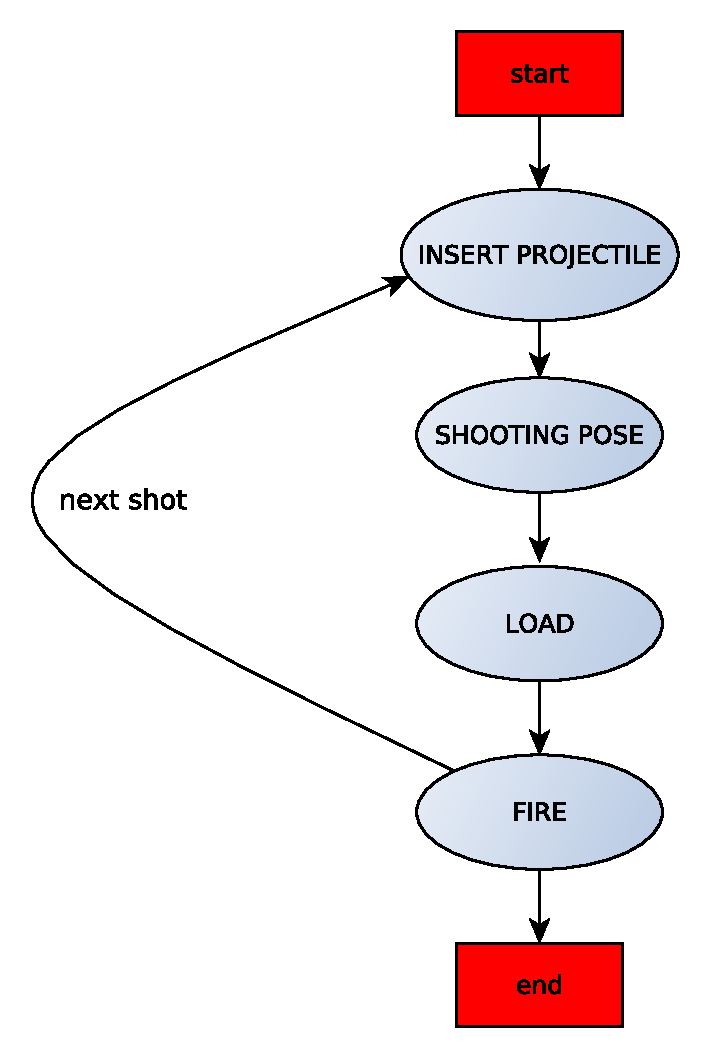
\includegraphics[height=0.5\textheight]{SlingshotStateMachine.pdf}						\centering
			\caption{Slingshot workflow.}
			\label{fig: slingshot workflow}
			\end{figure}


			\begin{figure}
			\includegraphics[width=0.25\textheight]{slingshot_process.png}			
			\centering
			\caption{Slingshot process diagram -- the top view.}
			\label{fig: slingshot process}
			\end{figure}		
			
			The flow chart connected with the shooting process is shown in Figure~\ref{fig: slingshot process}.
				
			\paragraph{Insert the projectile}~\\
				\indent The projectile is inserted into the gripper manually.
				
				A little trick is used to simplify this procedure for the operator. Normally, the operator presses a button to close the gripper. But when the operator enters the safety cage with the robot to insert the projectile, it is hard to reach the keyboard. Therefore, the gripper closes, when the force exerted on it exceeds a certain threshold. Thus, no keyboard is needed to close the gripper after the projectile has been inserted (see Figure~\ref{fig:ProjectileInsertion}).

				\begin{figure}
				\includegraphics[width=0.5\textheight]{ProjectileInsertionAdj.png}			
				\centering
				\caption{Inserting the projectile.}
				\label{fig:ProjectileInsertion}
				\end{figure}

				
			\paragraph{Shooting position (A)}~\\
				\indent The right arm of the robot moves next to the slingshot.
				
			\paragraph{Load (B, C)}~\\
				\indent The right arm holding the projectile moves towards the elastic string. The movement stops, when the projectile touches the string (B). It is detected by the force sensor in the right arm. When the force exceeds a certain threshold force $F_B$, the movement is stopped. The arm then moves a bit back (C).
				
			\paragraph{Fire (D)}~\\
				\indent The right arm moves backwards (D) until the desired force $ F_D$ is reached. Then the gripper opens and the projectile is released.

		\subsection{Force/torque sensor}
			In order to implement projectile insertion, loading and firing, a force feedback is needed. There are two ATI Mini 45 force sensors placed in the wrist of each arm. The force sensor measures the force and torque simultaneously in three axes. Thus, it provides $F_{x, y, z}$ and $T_{x,y,z}$ at the maximum frequency of \SI{7,000}{Hz}. After the filtration of the outside disturbances (such as trams and light disturbances) and subtracting the weight of the gripper, the sensor provides the meaningful data at the frequency of \SI{12.5}{Hz}~\cite{KubesForceSensor}. I use the force measurements only.
	
	
	\section{Experimental setting}

		\subsection{Shooting scene}
		
			Figure~\ref{fig:shooting setting} shows two settings of the shooting with the slingshot. The left diagram shows the horizontal shooting, the right one the shooting upwards. The shooting parameters were $z_0 = $ \SI{1.9}{m}, $ d = $ \SI{1.85}{m}.
			
			\begin{figure}[h]
			\centering
			\begin{tabular}{cc}
			\includegraphics[width=0.48\textwidth]{horizontal.png}
			%
			&
			%
			\includegraphics[width=0.48\textwidth]{askew.png}
			\end{tabular}
			\caption{Left: Shooting horizontally. Right: Shooting upwards.}
			\label{fig:shooting setting}
			\end{figure}
			
	
		\subsection{Projectile}
			A bent piece of wire was chosen to be the projectile (see Figure~\ref{fig: projectile}) for the following reasons. Firstly, the gripper can hold it, even if a high force is exerted on it. Secondly, it is light and finally, because it has a low air resistance.

			\begin{figure}[h]
			\includegraphics[width=0.5\textwidth]{bulletAdj.png}			
			\centering
			\caption{The projectile.}
			\label{fig: projectile}
			\end{figure}
			
			The weight of the projectile $m$ was measured to be in the range~1 to~\SI{2}{g}.
			
			When the projectile is shot, it leaves the slingshot with the initial velocity $ v_0$. Its magnitude is given by Equation~\eqref{eq: v0} and is derived assuming that the potential energy of the elastic string $ E_p$ is fully converted into the kinetic energy of the projectile $ E_k$. The diagram connected to shooting the projectile is shown in Figure~\ref{fig: shooting projectile}.
			
\begin{align}
E_p & = E_k \\[1ex]
%
\frac{1}{2}F \Delta x & = \frac{1}{2} m v_0^2 \nonumber \\[1ex]
%
v_0 & = \sqrt{\frac{F \Delta x}{m}}
\label{eq: v0}
\end{align}	
			
			The distance $ \Delta x$ is measured from the moment the force sensor detects a non-zero force until the moment when the desired force is reached.
			
			\begin{figure}
			\includegraphics[width=0.35\textwidth]{force.png}			
			\centering
			\caption{Shooting the projectile.}
			\label{fig: shooting projectile}
			\end{figure}

	\section{Implementation}

		\subsection{Force feedback}	

			A key task is to use the force feedback. Force thresholds $F_B$ and $F_D$ are used to detect hitting the elastic string (B) and to detect reaching the firing position, respectively. In addition, the force threshold $F_{D0}$ is used to detect that the elastic string starts to be stretched. This information is used to compute the distance $\Delta x$.

		\subsection{Traditional slingshot} \label{sec: implementation of slingshot 1.0}
		The slingshot script version 1.0 is called the shooter. The usage of the force feedback is implemented incrementally. It means that the arm moves a certain distance (e.g. \SI{1}{cm}) and then the force data is retrieved and checked whether it exceeds a certain force threshold. If not, another step is performed and the whole procedure is repeated. It results in a bit jerky movement of the robotic arm.
	
	\section{Mathematical description}
	
		The assumptions for the following mathematical description are the following.
%		
\begin{enumerate}\itemsep0pt
			\item The projectile is considered to be a point mass.
			\item The projectile has no air resistance.
			\item It is assumed that the motion takes place in a homogeneous gravitational field.			
\end{enumerate}	
		
		\subsection{Shooting horizontally}			
			
			Using the assumptions 1 and 2, the kinematics of the horizontal shooting is given by the two following Equations \eqref{eq: horizontal x} and \eqref{eq: horizontal z}. It is connected with the left side of Figure~\ref{fig:shooting setting}.
		
			\begin{equation} \label{eq: horizontal x}
				x = v_0 t
			\end{equation}
			\begin{equation} \label{eq: horizontal z}
				z = z_0 - \frac{1}{2} g t^2
			\end{equation}
			
			The time $ t_1$, in which the projectile hits the point $P_1 =  [x_1, z_1] = [d, z_1]$ on the opposite wall, is given by:
			
			\begin{equation}
				t_1 = \frac{d}{v_0}
			\end{equation}
			
			The z-coordinate $ z_1$ is then:
			
			\begin{equation} \label{eq: horizontal z1}
				z_1 = z_0 - \frac{1}{2}g t_1^2 = z_0 - \frac{g d^2}{2 v_0^2}
			\end{equation}
		
		\subsection{Shooting upwards}
		
			The setting of the shooting upwards corresponds to the right side of the Figure~\ref{fig:shooting setting}. Its kinematics is given by Equations \eqref{eq: upwards x} and \eqref{eq: upwards z}.
			
			\begin{align}
				x = v_0 \, t \, \cos \alpha \label{eq: upwards x} \\
				z = z_0 + v_0 \, t \, \sin \alpha - \frac{1}{2}g t^2 \label{eq: upwards z}
			\end{align}
			
			The time $ t_1$, in which the projectile hits the point $P_1 =  [d, z_1]$ on the opposite wall, is given by:
			
			\begin{equation}
				t_1 = \frac{d}{v_0 \, \cos \alpha}
			\end{equation}
			
			The z-coordinate $ z_1$ is then:
			
			\begin{equation} \label{eq: upwards z1}
				z_1 = z_0 + v_0 \, t_1 \, \sin \alpha - \frac{1}{2}g t_1^2 = z_0 + d \, \tan \alpha - \frac{1}{2}g t_1^2
			\end{equation}
			

				
	\section{Experiments with the traditional slingshot}
	
		\begin{figure}[h]
		\centering
		\begin{tabular}{cc}
		\includegraphics[height=111px]{string_horizontal.png}
		%
		&
		%
		\includegraphics[height=111px]{string_upwards.png}
		\end{tabular}
		\caption{Left: Straight elastic string ($ \alpha = 0$). Right: Bent elastic string ($ \alpha > 0$).}
		\label{fig:shooting string}
		\end{figure}		
	
		\subsection{Shooting horizontally}
			The first shooting experiment was conducted with a completely straight tightened elastic string. Thus, $ \alpha = 0$ and the projectile was shot horizontally. Figure~\ref{fig:shooting string}	left shows the side view of the slingshot.
			
			The projectile was shot in the following setting: $ F_1 = $ \SI{4.4}{N}, $ \Delta x = $ \SI{0.05}{m}. The shot hit the wall at the height $ z_1 = $ \SI{0.5}{m}. Thus, the initial velocity $ v_{01d}$ was \SI{10.49}{ms^{-1}} according to Equation~\eqref{eq: v0}.
			
			It is possible to estimate the initial velocity from the point $ P_1 = [d, z_1]$. Using Equations~\eqref{eq: horizontal x} and \eqref{eq: horizontal z}, we obtain:
			
			\begin{equation}
				v_0 = d \: \sqrt{\frac{g}{2(z_0 - z_1)}}
			\end{equation}
			
			In our case, $ v_{01k} = $ \SI{3.46}{ms^{-1}}.
			
			Thus, there is a substantial difference (roughly three times) between the initial velocity $v_{01d}$ (calculation based on the parameters of the elastic string and its dynamics) and the initial velocity $v_{01k}$ (calculation based on the kinematics of the horizontal shooting). This suggests that the theoretical model does not fit with the reality.
			
		\subsection{Shooting upwards}
			To make the shooting look as shooting and not as a ``piece of wire falling down'', $ \alpha$ was set to be higher than zero. I accomplished this by moving the elastic string a bit to the side (see Figure~\ref{fig:shooting setting} right). Parameters $ a = $ \SI{6}{cm} and $ c = $ \SI{6.1}{cm} yield:
			\begin{equation}
				\alpha = \arccos \left(\frac{a}{c} \right) \approx 10^{o}
			\end{equation}
			
			Given $ F_1$ and $ \Delta x$, the z-coordinate $ z_1$ of the point $ P_1$ can be computed using Equation~\eqref{eq: upwards z1}). However, the theoretical calculation is very sensitive to the change in $ \alpha$ and $ \Delta x$. Table \ref{table: change in alpha} shows how the change in $ \alpha$ (given $\Delta x = $ \SI{7}{cm} and $F_1 = $ \SI{4.8}{N}) influences $z_1$. Table \ref{table: change in dx} shows how the change in $ \Delta x$ (given $ \alpha = 10^{o}$ and $F_1 = $ \SI{4.8}{N}) influences $z_1$.

			\begin{table}\centering
			\ra{1.3}
			\begin{tabular}{@{}cc@{}}\toprule
			$\alpha$ [$^{o}$] & $ z_1$ [\SI{}{cm}] \\ \midrule
			
			5  & 105 \\
			10 & 120 \\
			15 & 132 \\
			20 & 144 \\
			 \bottomrule
			\end{tabular}
			\caption{Change in $\alpha$.}
			\label{table: change in alpha}
			\end{table}
			
			\begin{table}\centering
			\ra{1.3}
			\begin{tabular}{@{}cc@{}}\toprule
			$\Delta x$ [\SI{}{cm}] & $ z_1$ [\SI{}{cm}] \\ \midrule
			
			5 & 78 \\
			6 & 102 \\
			7 & 120 \\
			8 & 132 \\
			9 & 142 \\
			\bottomrule
			\end{tabular}
			\caption{Change in $ \Delta x$.}
			\label{table: change in dx}
			\end{table}
			
			The actual $ \Delta x_1$ and $F_1$  were measured to be $\Delta x_{1m} = $ \SI{5}{cm} and $F_{1m} = $ \SI{4.8}{N}. The shots were oscillating around the height $z_{1m} =$ \SI{150}{cm}.
			
			The theoretical $z_{1t}$ corresponding to the measured $\Delta x_{1m}$ and $F_{1m}$ is $z_{1t} = $ \SI{78}{cm}.
			
			To achieve the measured $z_{1m}$ given $F_{1m}$, $ \alpha$ and $\Delta x$ would have to be e.g. $\alpha_t = $ \SI{25}{\degree} and $\Delta x_{1t} = $ \SI{7}{cm}.
			
			A video called \textit{TraditionalSlingshot.mpg} was taken that shows the whole shooting procedure. It can be found on the attached CD.

	
	\section{Experiments with the flat slingshot}
		The previous experiments with the traditional slingshot had one problem. It was not possible to attach the traditional slingshot to the robot, so that it does not move while shooting. This behavior means that it is not possible to measure the shooting angle $\alpha$ properly and thus it is not possible to compare the measured results with the theoretical analysis.

		Therefore, a new slingshot model was introduced -- ``flat slingshot'' (see Figure~\ref{fig:flat slingshot}). It is made from plank wood. Its sides are flat and thus it is possible to attach it tightly to the arm of the robot.

		\begin{figure}
		\includegraphics[width=0.5\textwidth]{attached_flat_slingshot.png}			
		\centering
		\caption{The flat slingshot.}
		\label{fig:flat slingshot}
		\end{figure}

		\subsection{Changes to the traditional slingshot}
			The shooting procedure was changed a bit as well compared to the original one, see Section~\ref{subsec: traditional workflow}. The insertion of the projectile and moving to the shooting position was flipped.

			Secondly, the implementation of loading and firing was changed, see Section~\ref{sec: implementation of slingshot 1.0}, as well. The motion of the robotic arm is no longer jerky as it was before. Now the arm does not move incrementally in \SI{1}{cm} steps and does not check the measured force value only after one step was performed.  The smooth movement was achieved. However, the speed of the robot is slowed down ten times and the movement and force checking for threshold values are performed simultaneously. When the desired stopping threshold is reached, i.e. the projectile touches the elastic string, the movement is stopped immediately.

			Figure~\ref{fig: shooting process 2.0} shows the different states of the shooting procedure.

			\begin{figure}[h]
			\centering
			\begin{tabular}{ccc}
			\includegraphics[width=0.3\textwidth]{shooting_posAdj.png}
			%
			&
			%
			\includegraphics[width=0.3\textwidth]{loadAdj.png}
			%
			&
			%
			\includegraphics[width=0.3\textwidth]{fireAdj.png}
			\end{tabular}
			\caption{Left: Shooting position. Middle: Loaded. Right: Ready to fire.}
			\label{fig: shooting process 2.0}
			\end{figure}

		\subsection{Shooting at different shooting angles}
			The three following experiment were performed with the flat slingshot. Five shots were fired for different shooting angles $ \alpha_{1} = $ \SI{0}{\degree}, $ \alpha_{2} = $ \SI{10}{\degree} and $ \alpha_{2} = $ \SI{20}{\degree}. The height $ z $, shooting force $F$ and $\Delta x$ were measured. Table \ref{table: exp alpha 0}, \ref{table: exp alpha 10} and \ref{table: exp alpha 20} show the measured results. The shooting force $F_0$ was set to \SI{3.7}{N}.


			\begin{table}\centering
			\ra{1.3}
			\begin{tabular}{@{}cccc@{}}\toprule
			Trial & $z$ [m] & $F$ [N] & $\Delta x$ [m] \\ \midrule

			1 & 1.45 & 4.30 & 0.048 \\
			2 & 1.35 & 3.95 & 0.070 \\
			3 & 1.40 & 3.91 & 0.046 \\
			4 & 1.50 & 4.08 & 0.046 \\
			5 & 1.55 & 4.26 & 0.048 \\
		
			\bottomrule
			\end{tabular}
			\caption{Shooting 1: $\alpha = $ \SI{0}{\degree}.}
			\label{table: exp alpha 0}
			\end{table}

			\begin{table}\centering
			\ra{1.3}
			\begin{tabular}{@{}cccc@{}}\toprule
			Trial & $z$ [m] & $F$ [N] & $\Delta x$ [m] \\ \midrule

			1 & 1.70 & 4.98 & 0.049 \\
			2 & 1.65 & 4.40 & 0.049 \\
			3 & 1.70 & 4.12 & 0.052 \\
			4 & 1.75 & 4.45 & 0.047 \\
			5 & 1.65 & 4.26 & 0.050 \\
		
			\bottomrule
			\end{tabular}
			\caption{Shooting 2: $\alpha = $ \SI{10}{\degree}.}
			\label{table: exp alpha 10}
			\end{table}

			\begin{table}\centering
			\ra{1.3}
			\begin{tabular}{@{}cccc@{}}\toprule
			Trial & $z$ [m] & $F$ [N] & $\Delta x$ [m] \\ \midrule

			1 & 1.65 & 4.37 & 0.050 \\
			2 & 1.65 & 4.43 & 0.047 \\
			3 & 1.70 & 4.37 & 0.049 \\
			4 & 1.65 & 4.47 & 0.073 \\
			5 & 1.70 & 3.94 & 0.049 \\
		
			\bottomrule
			\end{tabular}
			\caption{Shooting 3: $\alpha = $ \SI{20}{\degree}.}
			\label{table: exp alpha 20}
			\end{table}

		\subsection{Comparison with the theoretically calculated values}

			For each trial, a theoretical height $z_{t}$ was computed according to Equations \eqref{eq: horizontal z1} and \eqref{eq: upwards z1}. Then a difference $ \Delta z = z_{m} - z{t}$ was computed for each trial. Tables \ref{table: exp comparison 1}, \ref{table: exp comparison 2}, \ref{table: exp comparison 3} show the obtained results.
			

			\begin{table}\centering
			\ra{1.3}
			\begin{tabular}{@{}cccc@{}}\toprule
			Trial & $ z_m$ [m] & $z_t$ [m] & $\Delta z$ [m] \\ \midrule

			1 & 1.45 & 1.09 & 0.36 \\
			2 & 1.45 & 1.29 & 0.06 \\
			3 & 1.40 & 0.97 & 0.43 \\
			4 & 1.50 & 1.00 & 0.49 \\
			5 & 1.55 & 1.08 & 0.47 \\
		
			\bottomrule
			\end{tabular}
			\caption{Shooting 1 comparison ($\alpha = $ \SI{0}{\degree}).}
			\label{table: exp comparison 1}
			\end{table}
			

			\begin{table}\centering
			\ra{1.3}
			\begin{tabular}{@{}cccc@{}}\toprule
			Trial & $ z_m$ [m] & $z_t$ [m] & $\Delta z$ [m] \\ \midrule

			1 & 1.70 & 1.51 & 0.18 \\
			2 & 1.65 & 1.42 & 0.23 \\
			3 & 1.70 & 1.42 & 0.28 \\
			4 & 1.75 & 1.40 & 0.35 \\
			5 & 1.65 & 1.48 & 0.17 \\
		
			\bottomrule
			\end{tabular}
			\caption{Shooting 2 comparison ($\alpha = $ \SI{10}{\degree}).}
			\label{table: exp comparison 2}
			\end{table}

			\begin{table}\centering
			\ra{1.3}
			\begin{tabular}{@{}cccc@{}}\toprule
			Trial & $ z_m$ [m] & $z_t$ [m] & $\Delta z$ [m] \\ \midrule

			1 & 1.65 & 1.70 & 0.05 \\
			2 & 1.65 & 1.66 & -0.01 \\
			3 & 1.70 & 1.69 & 0.01 \\
			4 & 1.65 & 1.99 & -0.34 \\
			5 & 1.70 & 1.59 & 0.11 \\
		
			\bottomrule
			\end{tabular}
			\caption{Shooting 3 comparison ($\alpha = $ \SI{20}{\degree}).}
			\label{table: exp comparison 3}
			\end{table}

			The results suggest that Trial 2 and Trial 4 in Shooting 1 and Shooting 3 are badly measured since $\Delta x$ is far off the other $\Delta x$ measured. These values were omitted in the following analysis.

			Finally, the means $\mu$ and standard deviations $\sigma$ were computed for the differences $ \Delta z$. Table \ref{table: exp analysis} shows the results.

			\begin{table}\centering
			\ra{1.3}
			\begin{tabular}{@{}ccc@{}}\toprule
			$\alpha^{o}$ & $\mu$ [m] & $\sigma$ [m]\\ \midrule

			0 & 0.44 & 0.06 \\
			10 & 0.24 & 0.07 \\
			20 & 0.02 & 0.07 \\
			
			\bottomrule
			\end{tabular}
			\caption{Statistical analysis of $\Delta z$.}
			\label{table: exp analysis}
			\end{table}

	\section{Discussion}

		\subsection{Traditional slingshot}
			The obtained results suggest that the theoretical model does not fit with the actual experiments. However, since it is not possible to attach the traditional slingshot tightly to the robotic arm, there is not much that can be done about it.

			However, the experiments show that a certain repeatability is indeed reachable. Out of six shots fired with a given force and shooting angle, three hit the target hanging on the wall. I recorded the whole experiment on video called \textit{TraditionalSlingshot.mpg} that can be found on the attached CD.

		\subsection{Flat slingshot}
			The results suggest that there is a systematic error difference between the theoretical computed heights $z_t$ and actually measured values $z_m$. As the shooting angle $\alpha$ was gradually increased, the difference between the theoretical and measured values decreased to values close to zero.

			The reason could be the fact that the projectile is not held ``horizontally'' in the left gripper, but slightly upwards. To compensate that the way the shooting angle is adjusted would have to change. It seems that it is not enough that the shooting angle is controlled only by the rotation of the left arm. The right one would have to turn accordingly as well. Another possibility would be to redesign the slingshot again. Instead of having the elastic string tightened vertically, it could be placed horizontally. The shooting angle would be then controlled solely by changing the position of the right arm.
		
		
	
			
			
			